\newpage
\section{Memory}
	Computer performance depends on the speed of the memory and the processor. DRAM (dynamic ram)is 10 to 100 times slower than processors.\\
	Computer memories are the combination of a small fast cheap memory and a slow large cheap memory. The cache is SRAM(static)(main memory). A cache hit is when memory is retrieved from the SRAM or it's a cache miss. The third level of memory is the hard disk(virtual memory).\\
	cache is physical memory. main memory. virtual.
	\paragraph{Average memory access time (AMAT)}
	\begin{equation}
		AMAT = t_{cache}+ MR_{cache}(t_{MM} + MR_{MM}t_{VM})
	\end{equation}
	MR= miss rate\\
	If a cache misses the data found will be copied to the cache.\\
	Two rules for what is in the cache: spatial and temporal locality. Spatial, means that when a word is copied to the cache it can also copy similar words. Temporal, means that if there is a cache miss that data will be copied to the cache because it might be searched for again.
	\subsection{Caches}
		Caches are organized as two-dimensional arrays. The rows are called sets, and the columns are called ways. Each entry in the array consists of a data block and its associated valid and tag bits. Caches are characterized by:
		\begin{enumerate}
			\item capacity C
			\item block size B and number of blocks, B = C/b
			\item number of blocks in a set N
		\end{enumerate}
	\subsection{Types of cache}
	\paragraph{Direct mapped cache}
		Each set in the cache contains one block(one data per address). Block one of main memory maps to the set 1 of the cache and so on until the last set in the cache, then the next block in MM maps to the first set in the cache again.
	\paragraph{N-way set}
		Each set contains N blocks. Have lower miss rates, but are slower and more expensive.
	\paragraph{fully associative} is a cache with only one set(B-way set).\\
	If a set is full when new data must be loaded, most of the time LRU(least recently used) block is deleted.
	\subsection{Multiple level caches}
	Most systems use multiple levels of caches. Each level is also from SPRAM but bigger and therefore slower.
	\subsection{Misses}
	The first request to a cache block is called a compulsory miss, because the block must be read from memory regard- less of the cache design. Capacity misses occur when the cache is too small to hold all concurrently used data. Conflict misses are caused when several addresses map to the same set and evict blocks that are still needed.
	
	
	\begin{multicols}{2}
		\subsection{Kaskadierung von RAM-Chips}
			\begin{center}
				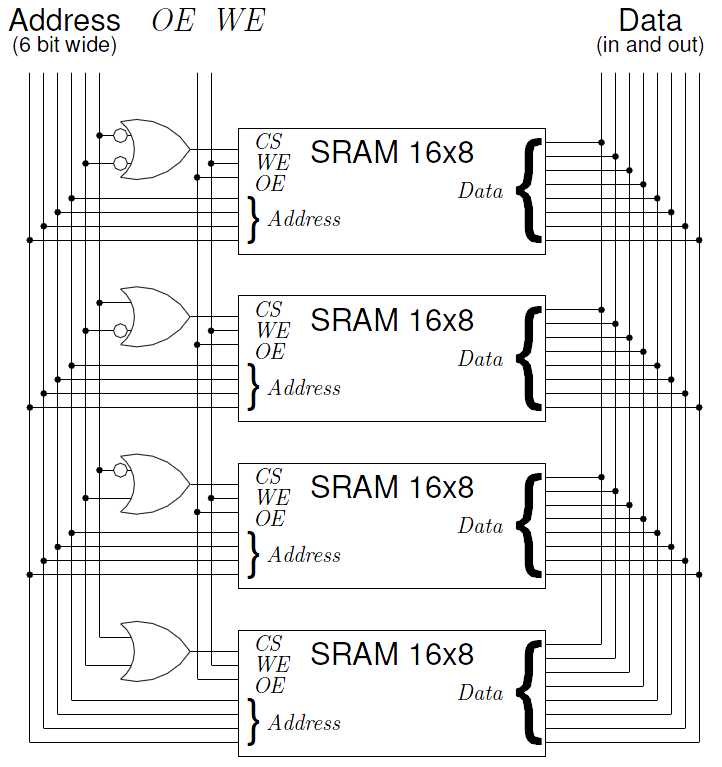
\includegraphics[width = 7cm]{images/mem/mem1.png}
			\end{center}
		ram looses it's memory when the power is turned off rom doesn't.
		
		
		\subsection{64 KBit (4096x16)}
			\begin{center}
			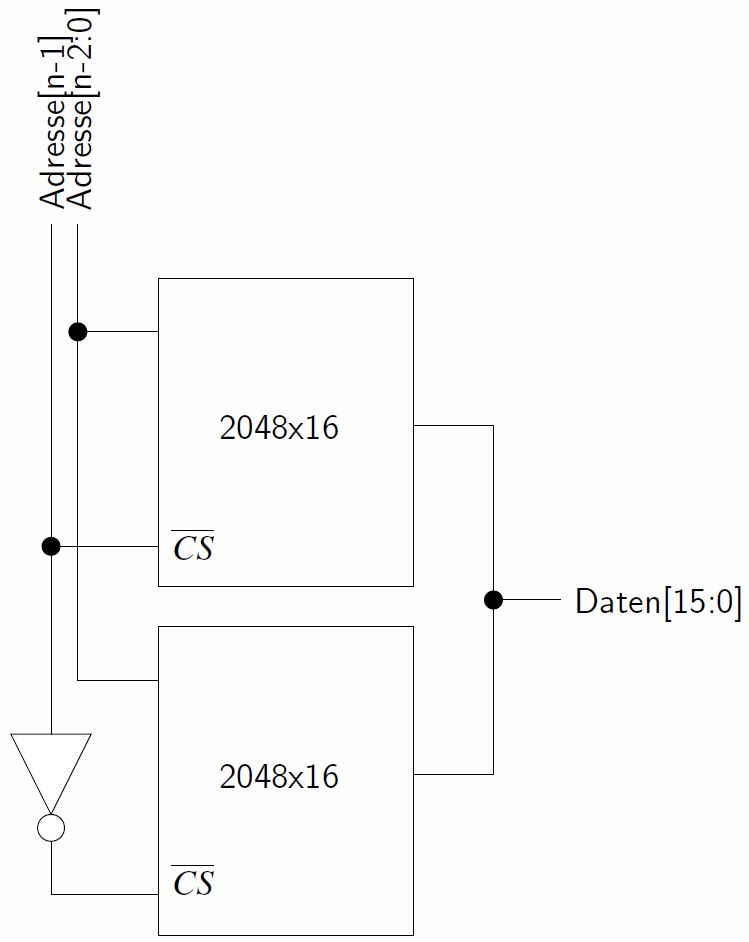
\includegraphics[width = 6cm]{images/mem/mem2-1.png}
			\end{center}
			
		\subsection{64 KBit (2048x32)}
			\begin{center}
			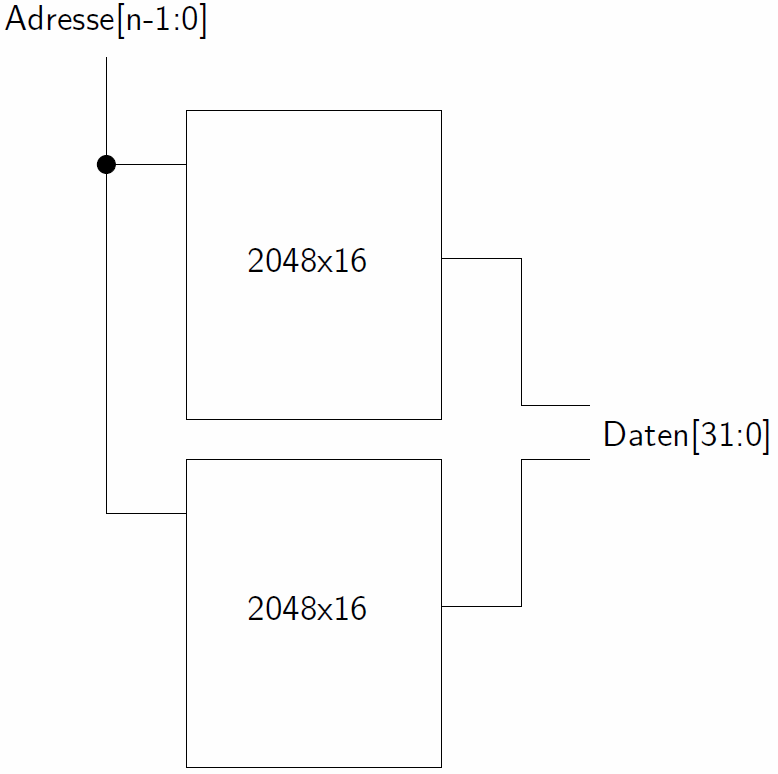
\includegraphics[width = 6cm]{images/mem/mem2-2.png}
			\end{center}
		
		\subsection{128 KBit (4096x32)}
			\begin{center}
			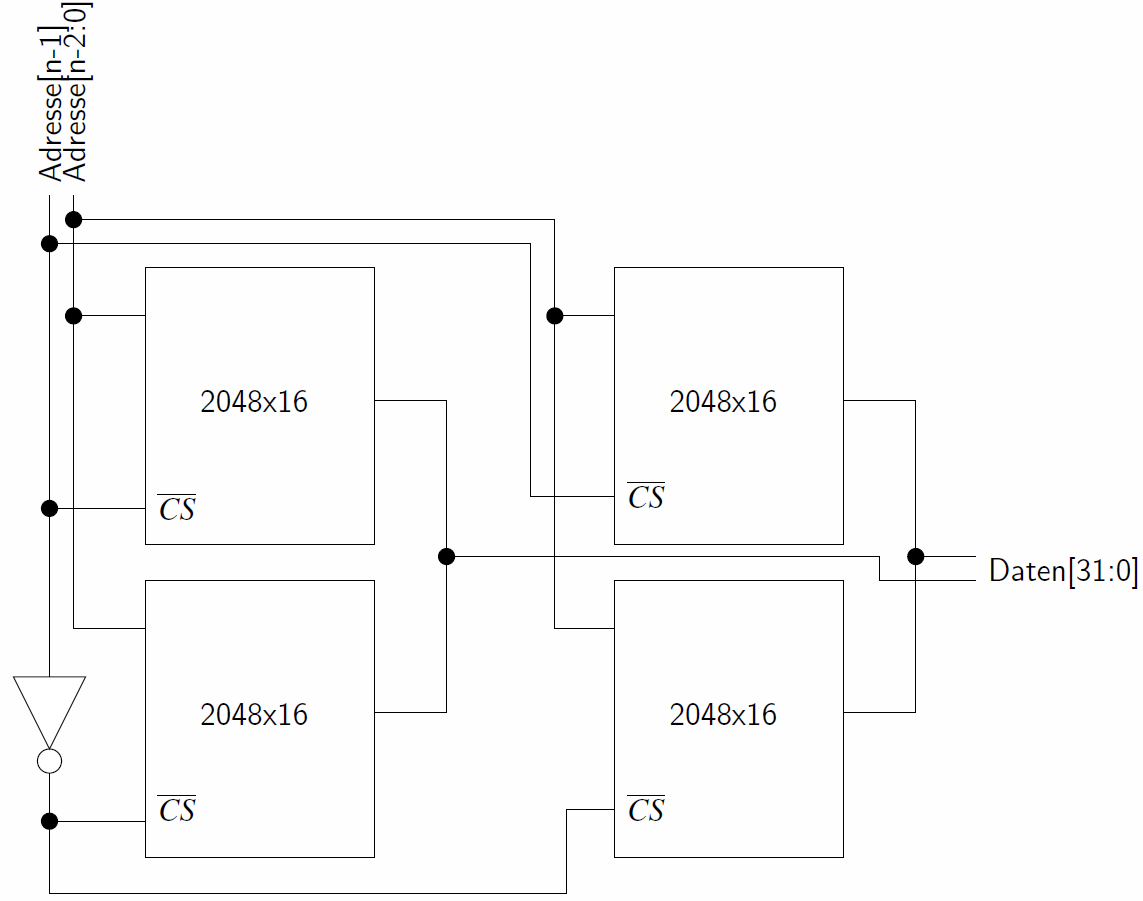
\includegraphics[width = 9cm]{images/mem/mem2-3.png}
			\end{center}
		

	\end{multicols}

	
\section{CMOS}
	\begin{multicols}{2}
			Es gibt zwei Schalttypen, NMOS und PMOS, beide werden aus Halbleitertransistoren aufgebaut.
			Dabei kommt dotiertes Silizium zum Einsatz, entweder p-dotiert (mit einem Überschuss an positiver Ladung)
			oder n-dotiert (zu viel negative Ladung).
			
			PMOS und NMOS Schalter dürfen nicht beliebig verbaut werden, ein NMOS-Transistor funktioniert nur zwischen
			\verb+out+ und \verb+GND+, während ein PMOS-Transistor nur zwischen \verb+VDD+ und \verb+out+ eingesetzt werden darf.
			
			\begin{center}
			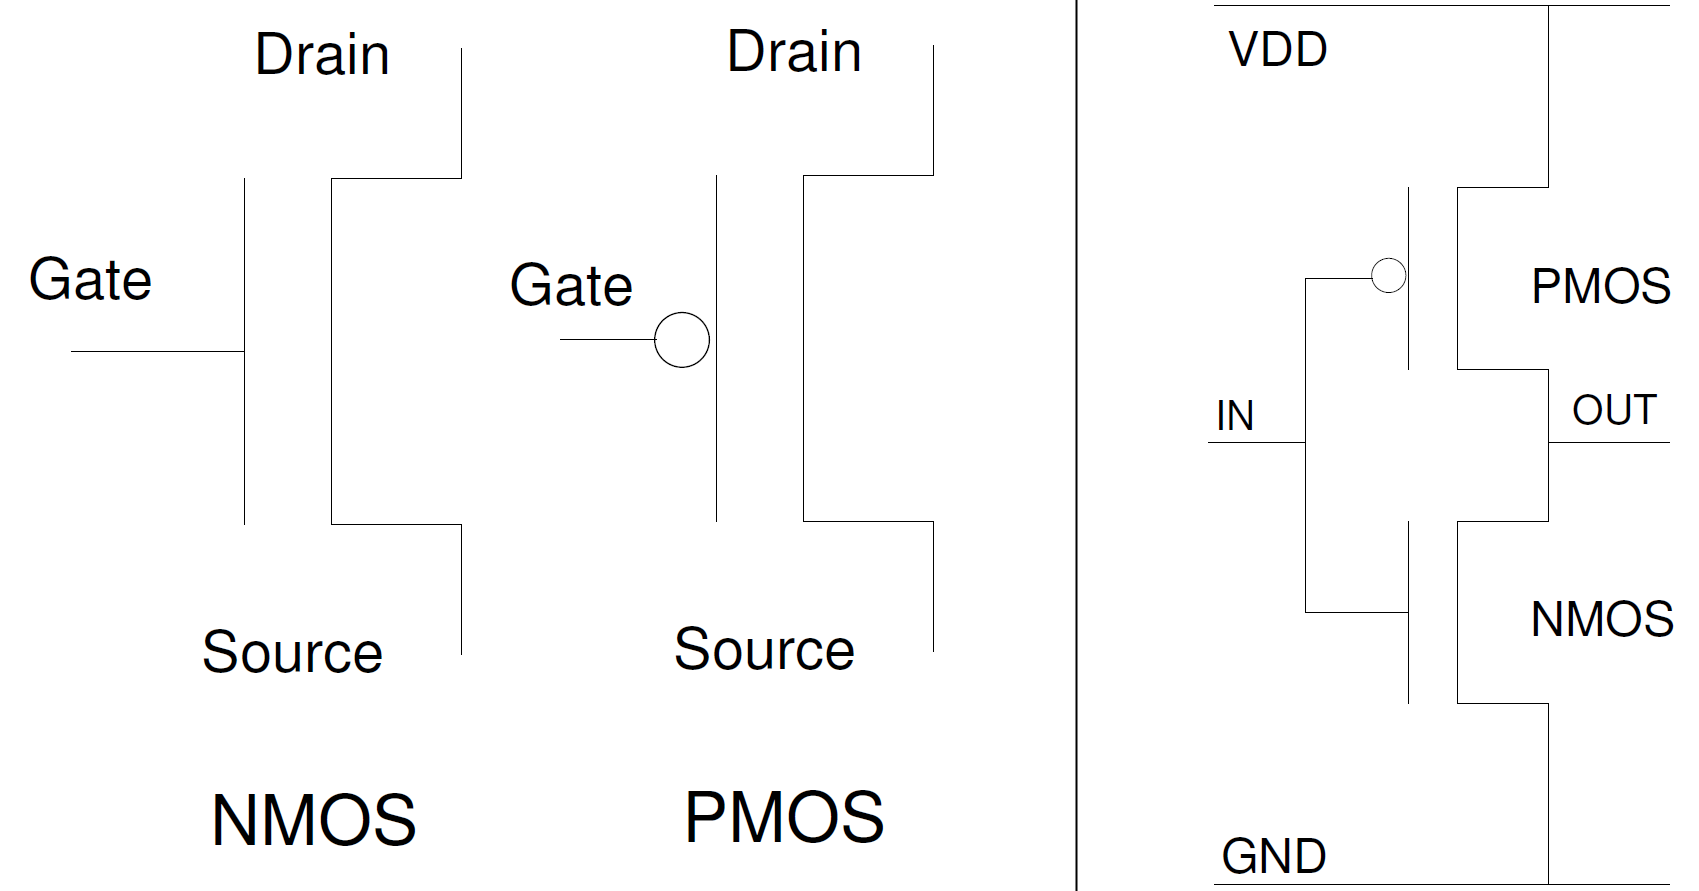
\includegraphics[width = 8cm]{images/mem/cmos.png}
			\end{center}
	\end{multicols}


















